
\section{Vene-vartion oma retki 3.–5.5.}


% \begin{multicols}{2}

\begin{multicols}{2}

\noindent \textit{Vene}"-vartio (aikaisemmin \mbox{\textit{Yllätysmunat}}) teki vartion oman retken Nuuksion Kyöpelille toukokuun alussa. Vartio kokoontui Leoa lukuun ottamatta lippukunnan varastolla, jossa retken yhteiset varusteet sekä osa ruoista pakattiin Mikon autoon. Loput retken ruoista ostettiin Pukinmäen S"-marketista, jossa pohdittiin, mitä tarkoittavat ''normaali paketti munia'' ja ''normaali pussi jauhoja''. Näiden selvittyä ja kun vartio saatiin täysvahvaksi, jatkui matka kohti Nuuksiota. Nuuksiontien päällystysurakka hidasti osastoa vähän, mutta perille päästiin huomattavasti nopeammin kuin julkisilla liikennevälineillä.

Ennakoiden lauantaina alkavaa maastopalovaroitusta (toim. huom. \textit{maastopalovaroitus} korvasi erilliset ruohikkopalo- ja metsäpalovaroitukset vuoden 2024 alusta), paistettiin makkarat jo perjantai"-iltana pian kämpälle saapumisen jälkeen. Tavanomaisia haasteita kohdattiin makkaran pysymisessä makkaratikussa -- etenkin, jos makkara oli viillelty. Haettiin vettä kaivolta sekä hakattiin -- ja välillä ehkä myös sahattiin -- polttopuita ansiokkaasti kämppäisännän toiveiden mukaisesti. Lauantain saunavuoroista sovittiin Korvenkolkalla retkeilevän lippukunnan aloitteesta.

\noindent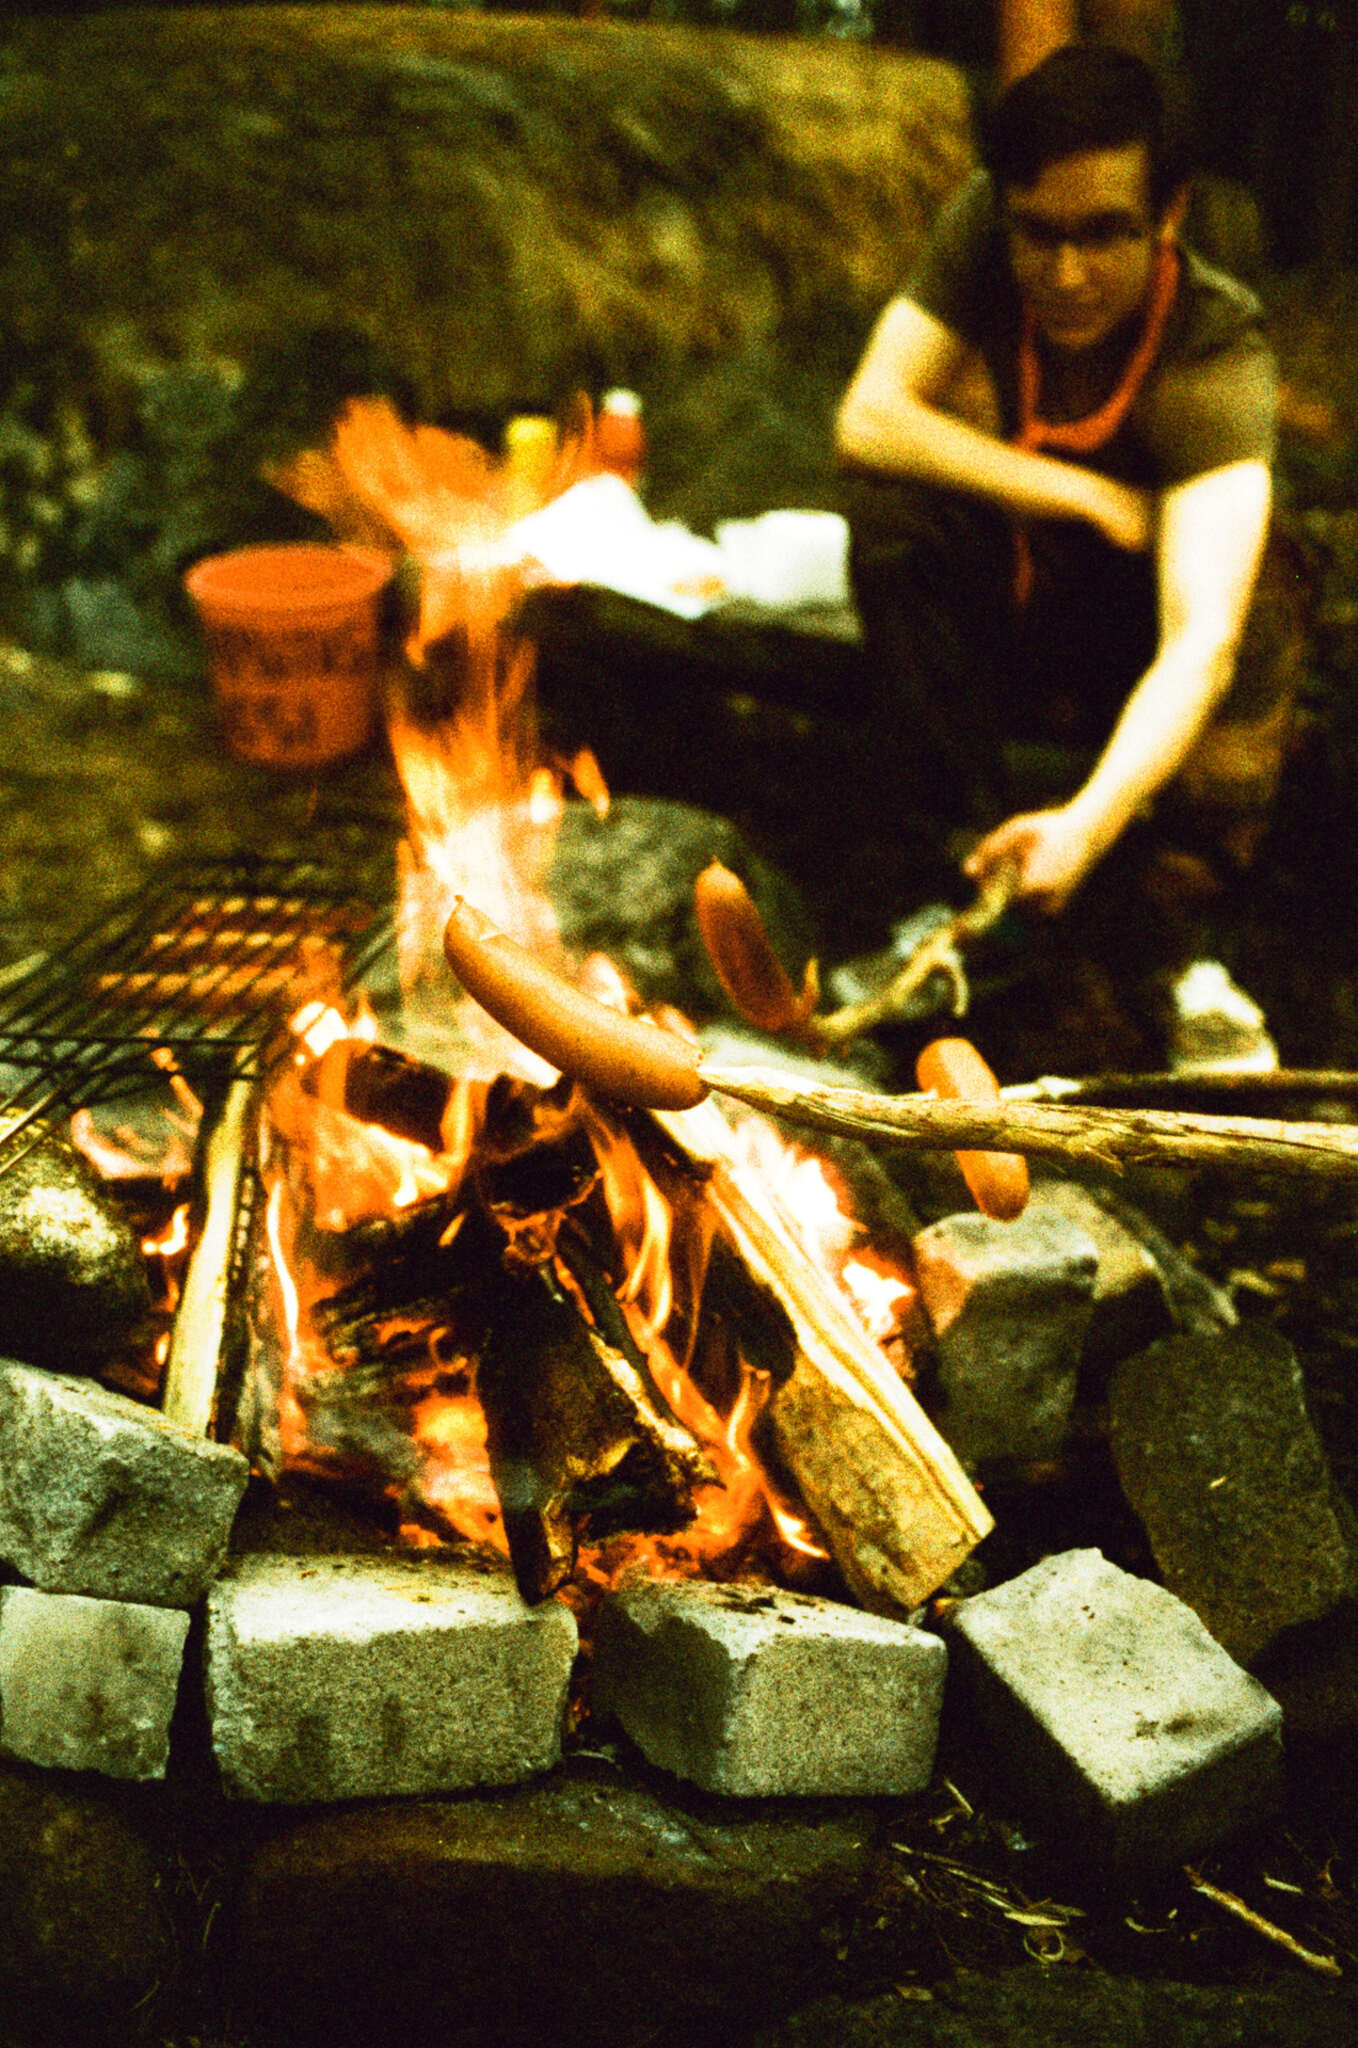
\includegraphics[width=\linewidth]{assets/vene05}

Lauantaina herättiin auringonpaisteeseen ja aamupäivä käytettiin pian tulevan lippukuntaretken suunnitteluun. Tämän lomassa allekirjoittanut kävi valmistelemassa iltapäivän suunnistuksen, hakattiin lisää polttopuita (tällä kertaa saunalle) ja urakoitiin pysäköintipaikkaa osoittavan liikennemerkin kanssa: Syystä tai toisesta vartio oli päättänyt irrottaa vanhan, puuvajan nurkilla lojuvan liikennemerkin siinä kiinni olevasta puolilahosta puupalkista. Ruosteinen mutteri ja asianmukaisten työkalujen puute tekivät harrastuksesta mielekkään pulmatehtävän. Lopulta mutterin sytyttimellä kuumentamisen ja monitoimityökalun pihtien rikkomisen jälkeen palkki saatiin kirveellä hakkaamalla liikennemerkistä irti.

Hernekeitto valmistui juuri sopivasti liikennemerkkihaasteen jälkeen. Pidettiin lyhyt ruokalepo ja oli aika iltapäivän suunnistukselle.

\vspace*{0.16cm}
\noindent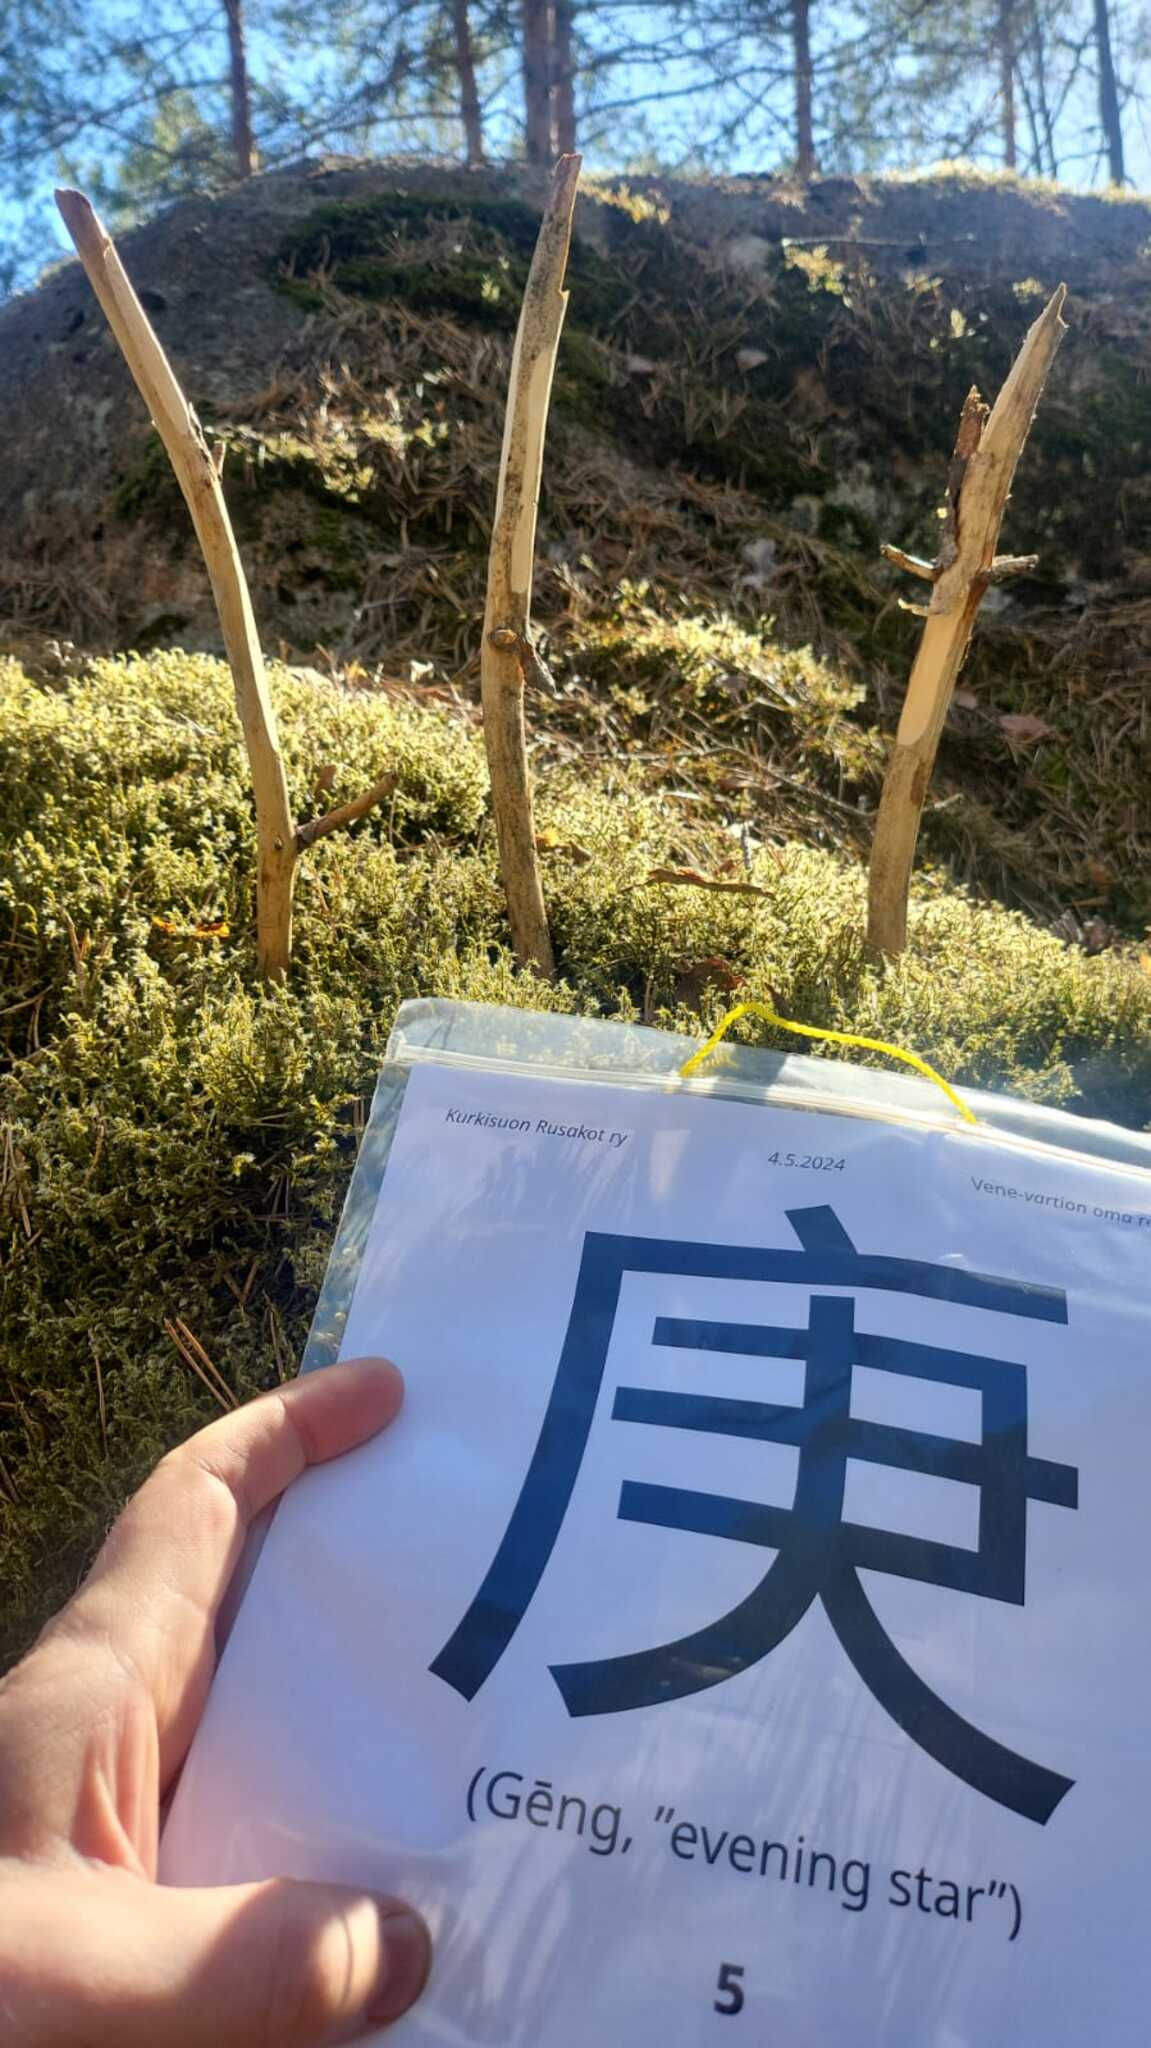
\includegraphics[width=\linewidth]{assets/vene11}

Jiǎ, yǐ, bǐng, dīng, wù\ldots\ Lauantai"-iltapäivän ohjelmassa oli tosiaan allekirjoittaneen \textit{Taivaalliset rungot} "=suunnistus, jossa \textit{Vene} pääsi harjoittelemaan niin suunnitustaitojaan kuin koordinaattien määritystä noin kuuden kilometrin radalla. Suunnistuksessa edettiin rastilta toiselle rastilipusta löytyvien koordinaattien perusteella ja kukin vartion jäsen suoriutui harjoitteesta varsin hyvin. Yksi milli kartalla vastasi kymmentä metriä maastossa, eli rastisijainnin määrityksissä sai olla tarkkana!

Suunnistuksen jälkeen toimitettiin nopea henkilökohtainen huolto ja nautittiin tonnikalanuudeleita. Halukkaat pääsivät saunomaan, mihin liittyen erityismainintana sekä vesipadan että kiukaan tulipesässä oli tuli vuoron alussa.

Kultaiset muistot taannoisen Bengtsårin Merisaunan retken musavisasta sai vartion innostumaan vastaavan järjestämisestä iltaohjelmana. Tällä kertaa visassa arvuuteltiin musiikkikappaleen nimen ja esittäjän lisäksi kappaleen alun sanoituksia, sanoituksia mielivaltaisessa kohdassa kappaletta, sanoituksista puuttuvaa sanaa, kappaleen nimeä sanoitusten hassunhauskan käännöksen avulla, kappaleen nimeä hyminän perusteella ja kappaleen nimeä pantomiimiesityksen perusteella. Kukin kilpailija sai valita viisi omavalintaista musiikkikappaletta, joita arvuuteltiin edellä mainituilla tavoilla. Pisteitä myönnettiin niin arvuuttelijalle kuin arvaajallekin. Valittujen kappaleiden kirjo oli arvatenkin hyvin laaja. Tällä kertaa musavisan voittajaksi selvityi Leo ylimääräisellä, ratkaisevalla kierroksella, jossa arvuuteltiin, kuinka seuraava kappale jatkuu: 

Älä tuu siihen droppaa mun tunnelmaa / Mitä eilistä juttua jankuttaa / Voitsä vetää suupielet ylöspäin / \ldots

Olisitko sinä tiennyt oikean vastauksen?

Musavisan uuvuttamat retkeläiset eivät enää jaksaneet paistaa lettuja, joten lettutaikinasta paistettiin paksu pannukakku iltapalaksi ja mentiin nukkumaan.

Suununtaipäivään ei oltu suunniteltu mitään erityistä ohjelmaa. Kämppä ja sauna siivottiin siivousohjeiden mukaisesti ja lähdettiin kotimatkalle. Vartiolla oli retkellä sen verran hauskaa, että puhuttiin seuraavan vartion oman retken järjestämisestä taas syksyllä!

\noindent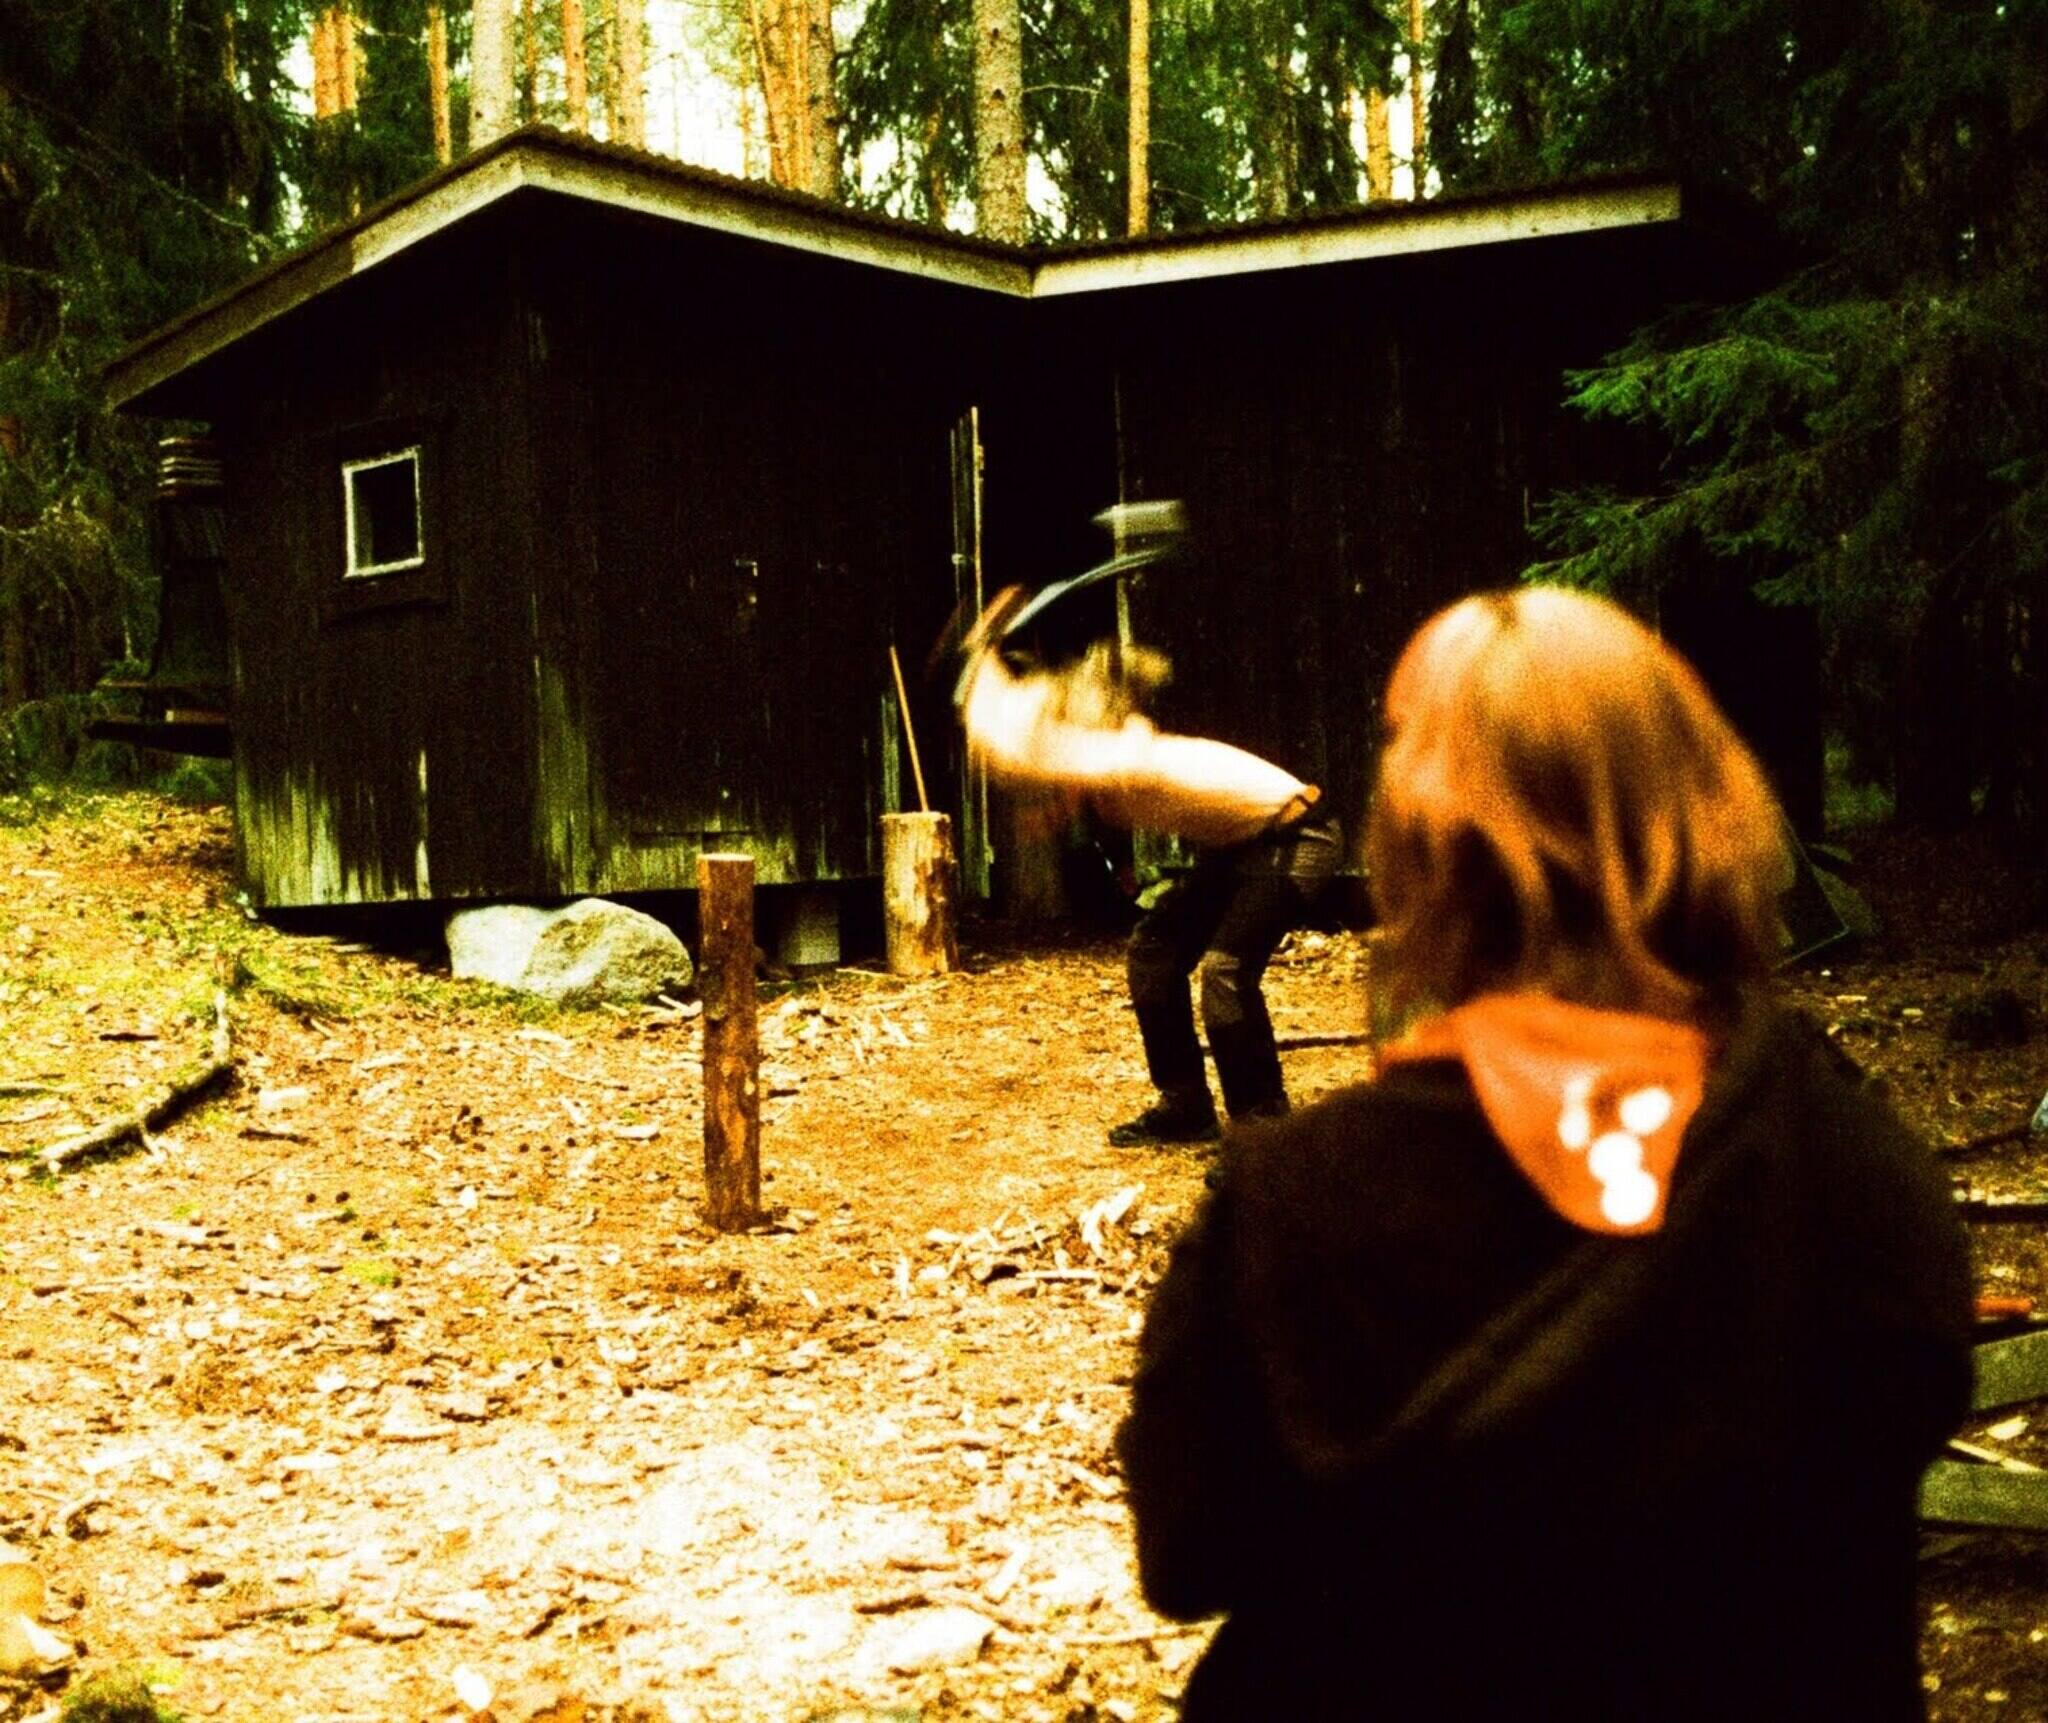
\includegraphics[width=\linewidth]{assets/vene02}

\begin{center}
\begin{tabular}{ |l|l| }
	\hline
	Ahti & 12 pistettä \\
	\hline
	Elias & 8 pistettä \\
	\hline
	Janne & 5 pistettä \\
	\hline
	\textbf{Leo} & \textbf{13 pistettä} \\
	\hline
	Mikael & 6 pistettä \\
	\hline
	Mikko & 10 pistettä \\
	\hline
\end{tabular}
\end{center}

\end{multicols}

{\raggedleft Kuvat: Janne Suomalainen \& Vene\\ Teksti: Janne Suomalainen\par}

\vspace*{0.32cm}
\vspace*{0.16cm}
\noindent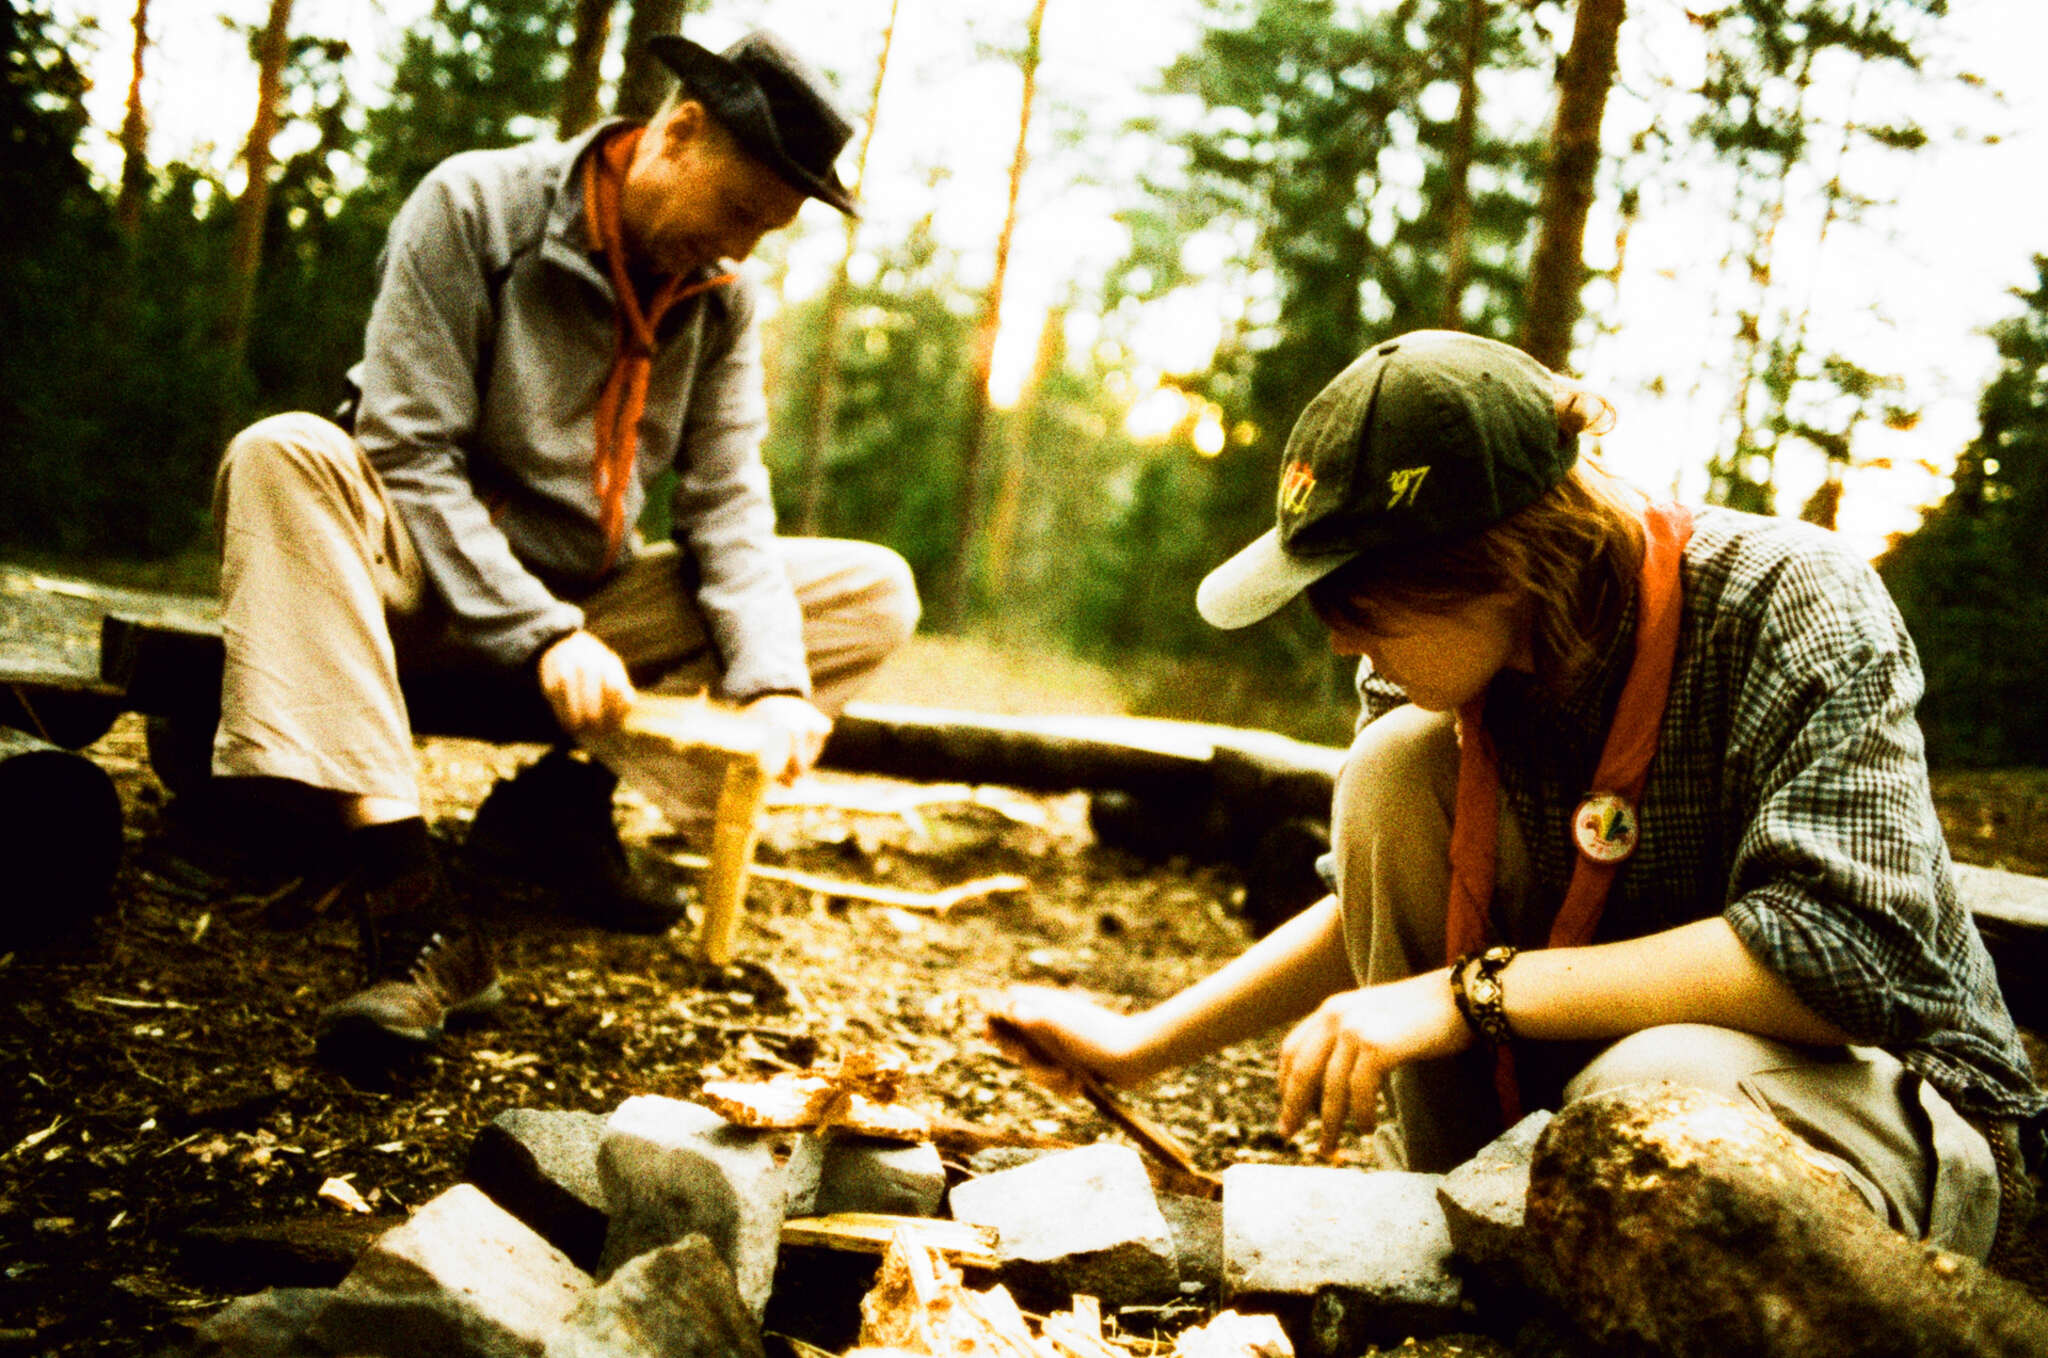
\includegraphics[width=\linewidth]{assets/vene03}
